\chapter{The $\lambda$-calculus and Curry Type Assignment System Implementation in Java}
The Java version of implementation is transferred directly from Haskell. However, the semantics and operational order of Haskell is difference from Java, especially the `where' statement of Haskell. The 'where' declaration is called when the defined variables are used, however, in Java, we need to separate a `where' block into parts according to where it is called. An example is shown in Section \ref{sec:hj}. This differece is worth taking care of when transfer the Haskell into Java, otherwise, NullPointerException may occur. 

In all data types, the method toString() has been implemented -- more precisely overridden, as it is a method of the Java primary class\verb| Object|. This function is used to print out the data type as a string. There are more method signatures defined in the interfaces as a reference to instantiable classes. 

\section{Different operational order between Haskell and Java}{\label{sec:hj}}
As mentioned above, the operaional order of Haskell is different from Java, not only the pattern matching, but also the `where' declarations. Since the code in Haskell cannot be transferred into Java directly, it largely abandoned the simplicity of codes. Following is a piece of code that defines principle pair algorithm:
\begin{verbatim}
ppc :: Term -> [Char] -> (PPc, [Char])
ppc (Abs x y) r | contains (Var x) pi = ((removeItem (Var x, a) pi,    <1>
                                         (TP a p)), tl1)
                | otherwise = ((pi, (TP f p)), tl1)                    <2>
                            where (f, tl) = fresh r                    (1) 
                                  ((pi, p), tl1) = ppc y tl            (2)
                                  (_, a) = search (Var x) pi           (3)

\end{verbatim}

Recall that, local definition is visible across the guards. `Guards' is used as an if-then-else block. In the example above, there are three declarations in the `where' block, each with a distinct number. For the first condition of \texttt{ppc} function, declaration (1)(2)(3) are called since all the declared variables in `where' block are used. In the `otherwise' function clause, only declaration (1)(2) are called. In this case, in order to transfer the Haskell function into Java methods, we need to repetitively define the variables which largely reduces the simplicity and conciseness of codes. 

Following is the corresponding Java method that implements the principal pair algorithm for abstractions:

\begin{verbatim}
public PPC ppc(Term term, String counter){
     ...
     else if(term instanceof Abstraction){
        Variable xv = new Variable(((Abstraction) term).getName());
    
        if(receiver != null){
    <1>    if(contains(xv, receiver.getSubject())){
    (1)      TVar f = new TVar(counter.substring(0, 1));
    (2)      PPC receiver = ppc(((Abstraction) term).getTerm(), counter.substring(1));
    (3)      Type searchType = search(xv, receiver.getSubject()).getPredicate();
             ArrayList<Statement> original = receiver.getSubject().getContext();
             ArrayList<Statement> remove = new ArrayList<>();

             for(Statement s: original){
               if(s.getSubject().equals(xv)) remove.add(s);
             }

             for(Statement rm: remove){
                original.remove(rm);
             }

             TP tp = new TP(searchType, receiver.getPredicate());
             return new PPC(new Context(original), tp, receiver.getCounter());
          }
    <2>    else{
    (1)      TVar f = new TVar(counter.substring(0, 1));
    (2)      PPC receiver = ppc(((Abstraction) term).getTerm(), counter.substring(1));
             return new PPC(receiver.getSubject(), new TP(f, 
                             receiver.getPredicate()),
                             receiver.getCounter().substring(1));
          }
       }
       else {
           return null;
       }
     }
     ...
}
\end{verbatim}

As labelled \verb|<1> <2>| in the code, which stands for the Java block corresponding to the Haskell functional clause. We can clearly see that the Haskell code is much more concise. Moreover, in Java, the declaration of the variables in \texttt{(2)} is redundant. Although it would not be executed if the outer condition is not satisfied, it decreases the readability of programs. Also, to remove an element in \verb|ArrayList| in Java is expensive. When we traverse through the \verb|ArrayList|, the element we are look for cannot be concurrently removed. Otherwise, it would cause the \verb|ConcurrentModificationException|. We need to create a recorder to record which element needs to be removed in the \verb|ArrayList| and remove them after the iteration.  

\section{$\lambda$-calculus Representation}
\subsection{$\lambda$-terms}
A Lambda term can either be a variable, an abstraction or an application. An interface `Term' is defined as a reference type, which has three lambda term implementations. This is the generic representation of all lambda terms.

\begin{figure}[ht]
\centering
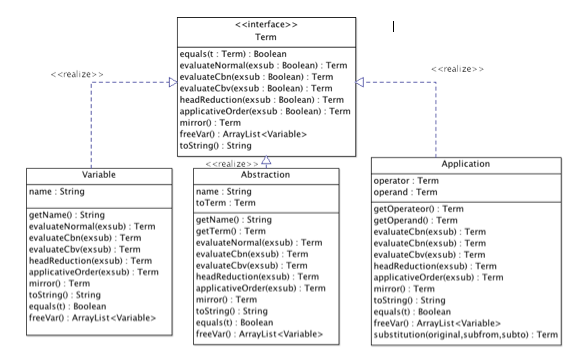
\includegraphics[scale=0.8]{pics/Term2}
\caption{Class diagram of Lambda Calculus data structures}
\label{fig:term1}
\end{figure}

Notice that, in Haskell, the name of a variable and the input of an abstraction are both single characters(in Section \ref{sec:reductionstrategy}). It only enables $\alpha$-conversion by renaming the bound variable to $z$. The problem arises when the variable $z$ is already used. In Java implementation, we make the name of a variable and the input of an abstraction become a string. The string is in the format \texttt{xn} where \texttt{x} is a single character and \texttt{n} is a number that can be regarded as the \texttt{id} of that variable. When we perform $\alpha$-conversion on a bound variable, we can simply increase its \texttt{id} so the variable is renamed.  

This interface defines the method \verb|equals(Term t)|, which return a boolean states whether it is equal to the input term. This method overrides the \verb|equals(Object o)| method of the Java primary class \verb|Object|. It is essential in the reduction procedure, since we can decide whether a term is reducible by compare the term before reduction and after. If the term is the same as it before reduction, then it cannot be reduced. Therefore, we know when we can stop the reduction procedure.  

As mentioned in Section \ref{sec:reductionstrategy}, there are five reduction strategies enabled in the reducer. So there are five method signatures defined in the interface: \textsf{evaluateNormal(Bool exsub), evaluateCbn(Bool exsub), evaluateCbv(Bool exsub), headReduction(Bool exsub), applicativeOrder(Bool exsub)}. Each of these method refers to a specific reduction strategy as the method name. 

The method \textsf{mirror()} is used to create a mirror term with exactly the same class variables. This method is used when the substitution is performed. For example, if we have a lambda term $\lambda f.(\lambda x.f(xx))(\lambda x.f(xx))$, it is reduced to $\lambda f.f((\lambda x.f(xx))(\lambda x.f(xx)))$. If we do not create a mirror term of $(\lambda x.f(xx))$, both of these two $(\lambda x.f(xx))$ would refer to the same memory space. In other words, the abstraction $(\lambda x.f(xx))$ is used twice to form an application. Therefore, if operations performed on the function, it is also performed on the argument. It is essential to create a mirror term that separate those two terms although they look exactly the same.

The method \textsf{freeVar()} is used to get all the free variables of a $\lambda$-term. It is used to perform $\alpha$-conversion when we substitute bound variables in an abstraction. The free variables are defined in Definition \ref{eq:fv}.       

Finally, the \textsf{toString()} method of class \textsf{Object} is overridden to transform a lambda term to a string. 

Notice that, in the implementation class \verb|Application|, there is a \textsf{substitution(Term original, Term subfrom, Term subto):Term} method. It is used to substitute bound variables in an abstraction, which is an application function, to the argument. The first parameter of the method is the body of abstraction, the second argument states which bound variable could be substituted and the third argument states what it could be substituted to.

\subsection{Parser}
To allow interactions and inputs from users, the program needs to interpret the input term into a data structure in the system. Figure \ref{fig:inter} illustrates all the methods that used to interpret an input into a lambda term data structure.   

\begin{figure}[ht]
\centering
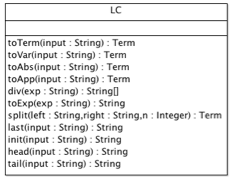
\includegraphics[scale=0.6]{pics/LC}
\caption{Interpretation methods in LC class}
\label{fig:inter}
\end{figure}

The method \textsf{toTerm(String input)} takes a string as input and returns a \textsf{Term}. It calls \textsf{toVar(String input), toAbs(String input)} or \textsf{toApp(String input)} according to type of the outermost term. Then, those three methods iteratively call each other until the whole term is interpreted.   

\textsf{div(String exp)} divides an application into the function and argument. Basically, it return an array with 2 string elements. The method \textsf{toExp(String exp)} is used to remove brackets of applications and returns an expression that is bracker-free. Finally, the most important method \textsf{split(String left, String right, Int n)} implements the bracket removal mechanism. It marks the right most right bracker `)' and find the matching left bracket `(' and extract the term out without brackets.

Since the Java implementation is directly transferred from Haskell, there are also four basic string operations which are Haskell builit-in functions. \textsf{last(String input)} takes a string and returns the last character of the string, it returns itself if the length of input string is 1. \textsf{init(String input)} accepts a string and returns the string without its last character, it returns an empty string if it only contains one character. \textsf{head(String input)} takes a string and returns the first element of the string, it returns itself when the input string length is 1. \textsf{tail(String input)} takes a string and returns the string without its first element, it returns an empty string when the length of input is 1. 

Following is the example of how those Haskell built-in function work:

\begin{verbatim}
              init "Hello"   "Hell"            head "Haskell"   "H" 
              init "A"       ""                head "A"         "A"
\end{verbatim}

\begin{verbatim}
              last "String"   "g"              tail "Lambda"   "ambda" 
              last "A"        "A"              tail "A"         ""
\end{verbatim}


\section{Curry Type Assignment System Representation}


\subsection{Types}{\label{subsec:types}}



Type assignment system assigns types to $\lambda$-terms. In $\mathbb{T}$, a type can either be a single type($A,B,...$) or a complex type($A\rightarrow B$). Since the complex type is formed by single types, it can be represented using the binary tree structure, where single types are leafs and complex types are branches. For example, the type $(A\rightarrow B)\rightarrow C$ is represented as \textsf{TP(TP (TVar A)(TVar B))(TVar C)}, or in a more intuitionistic way:

\Tree 
[.TP [.TP A B ] C ]

\begin{figure}[t]
\centering
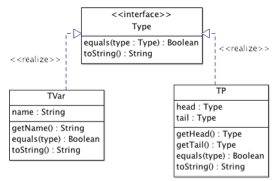
\includegraphics[scale=0.7]{pics/Type}
\caption{Class diagram of type representation}
\label{fig:type}
\end{figure}

Illustrated in Figure \ref{fig:type}, the interface \textsf{Type} is defined as a reference type. It defines two basic method signatures: \textsf{equals(Type type)} and \textsf{toString()} which override the primary methods in \textsf{Object}. There are two implementation class: \textsf{TVar} and \textsf{TP} which stand for single type and complex type. \textsf{TVar} contains a class variable \textsf{name} which states the type name. It implements method signatures defined in the interface and a get method that returns the type name. The implementation class \textsf{TP} is similar to a \textsf{Node} of a tree structure, which contains two class variables: left branch and right branch. Method signatures and get methods are implemented in the class.

\subsection{Type substitution}

Principal types for $\lambda$-terms are defined using the notion of unification of types that defined by Definition \ref{eq:rob}. Similar to types structure in Section \ref{subsec:types}, a type substitution can either be a single substitution($\varphi  \mapsto B$) or a complex substitution($S_1 \circ S_2$). It could also be represented as a binary tree structure. For example, when we unify $(A\rightarrow B)\rightarrow C$ and $(A\rightarrow D)\rightarrow E$, we would get the complex substitution$((A \mapsto A)\circ (B \mapsto D))\circ (C \mapsto E)$ which also can be represented as a binary tree:

\Tree 
[.So [.So $(A\mapsto A)$ $(B\mapsto D)$ ] $(C\mapsto E)$ ]

As shown in Figure \ref{fig:tsub}, an interface \textsf{TSub} is needed as a reference type. It doesnt have any method signatures, operation on substitutions are defined as auxiliary function in class \textsf{LC}.

\begin{figure}[ht]
\centering
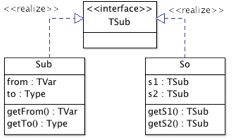
\includegraphics[scale=0.7]{pics/TSub}
\caption{Class diagram of type substitutions representation}
\label{fig:tsub}
\end{figure}
\subsection{Other data types}

The Curry type assignment system defines other concepts besides types and substitutions. Statement is essential to describe the type assigned to a $\lambda$-term; Context is used to collect all statements used for free variables of a term when typing that term; and PPC is a data type that stores context and the type assigned to that term typed. 

\begin{figure}[ht]
\centering
\begin{minipage}{.3\textwidth}
\centering
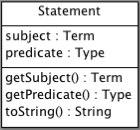
\includegraphics[scale=0.6]{pics/Statement}
\caption{Class diagram of Statement}
\label{fig:statement}
\end{minipage}\hfill
\begin{minipage}{.3\textwidth}
\centering
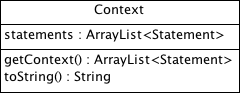
\includegraphics[scale=0.6]{pics/Context}
\caption{Class diagram of Context}
\label{fig:context}
\end{minipage}\hfill
\begin{minipage}{.3\textwidth}
\centering
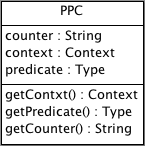
\includegraphics[scale=0.5]{pics/PPC}
\caption{Class diagram of PPC}
\label{fig:ppc}
\end{minipage}
\end{figure}

The \textsf{Statement} class has two attributes which are subject and predicate. It contains basic get method that return \textsf{private} attributes, and it also overrides the \textsf{toString()} method to transform a \textsf{Statement} into a string as ``subject : predicate''

The \textsf{Context} class only contains an \textsf{ArrayList} of \textsf{Statement} as attribute. A context could have none statement if all the variables are bound. The \textsf{toString()} method returns the context a string in the format: ``statement1, statement2, ...'' 

The \textsf{PPC} class, storing principle pair algorithm results, is a little more complex. As defined in Definition \ref{def:ppc}, the ppc function return a context and the type assigned to the term typed as $\langle$context, type$\rangle$. A PPC instance, stores the result of ppc function, therefore it contains two attributes as context and type. In additional, it also has a counter attribute. Since principle pair algorithm always create \textsf{fresh} types, we should keep track of what type names are available that have not been used. It basically states all the available type names.   

\subsection{Core type assignment mechanism implementation}

The Curry type assignment implementation is built based on the lambda calculus implementation. As it extends more operation on $\lambda$-terms for type assignment, there are more auxiliary methods defined in class \textsf{LC}. 

\begin{figure}[ht]
\centering
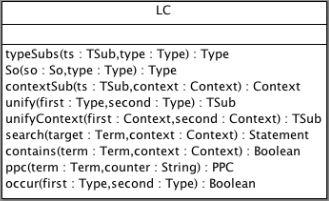
\includegraphics[scale=0.6]{pics/LCType}
\caption{Class diagram of Lambda Calculus data structures}
\label{fig:lctype}
\end{figure}


The methods listed in Figure \ref{fig:lctype} are the core type assignment mechanism implementations. The top-level method is \textsf{ppc(Term term, String counter)}, when a term comes in and needs to be typed, the ppc method is called and it iteratively calls other auxiliary methods. Finally, it will return a \textsf{PPC} instance which contains a context and the typed assigned. 

Given a type substitution and a type, the method \textsf{typeSubs(TSub, Type)} substitutes all the type variables according to the subsitution. It implements the type substitution defined in Definition \ref{def:tsub}. Notice that, since a \textsf{TSub} can either be a single substitution \textsf{Sub} or a complex \textsf{So} as defined in Section \ref{fig:tsub}, it calls \textsf{So(So, Type)} method that implements the \textsf{So} substitution described in Definition \ref{def:tsub} (b). 

The method \textsf{contextSub(TSub, Context)} implements the context substitution defined in Definition \ref{eq:rob} (c). 

The method \textsf{unify(Type, Type)} implements the type unification algorithm defined in Definition \ref{def:tsub}. And \textsf{unifyContext(Context, Context)} implements the context unification in Definition \ref{eq:rob} (ii). It should be mentioned that, since $Id_s$ stands for the substitution that replaces all type variables by themselves, it could be simplified as a substitution that only contains the substitution $(A\mapsto A)$. We do not care what the type $A$ is and whether it is a valid type variable, because the substitution $(A\mapsto A)$ would not affect any unifications. 

The \textsf{search(Term, Context)} methods is an auxiliary method that given a $\lambda$-term and a context, it returns the corresponding statement of that term in the context. This method is used in two places. Firstly, it is used when we want to unify the context $\Gamma_0$ and $\Gamma_1$. We need to find the statements with the same subject in these two context and unify them. Therefore, when we traverse through the context $\Gamma_0$, the search method is necessary to find the corresponding statement in $\Gamma_1$. Secondly, it is used in the principal pair algorithm when we type an abstraction. The temporary type assigned to bound variables should be removed from the context. Therefore, given a variable, the search method can find the corresponding statement and further be removed.  

The method \textsf{contains(Term, Context)} takes a $\lambda$-term and a context as arguments and return a boolean states whether the context contains a statement for the term.

\textsf{ppc(Term, String)} is the core principal pair algorithm implementation method. The definition of principal pair algorithm can be found in Definition \ref{def:ppc}. The second argument in \textsf{String} type is the counter of all available type names. 

Finally, the method \textsf{occur(Type, Type)} is used to decide whether a type occurs in another. It is used in the second type unification algorithm defined in Definition \ref{eq:rob}.

\section{Explicit substitution and garbage collection}

The lambda calculus with explicit substitution and garbage collection is built based on ordinary lambda calculus. The $\lambda$xgc-term has an additional $M\langle x:=N\rangle$ term compared to the lambda calculus. Therefore, in Figure \ref{fig:termxgc}, a new class \texttt{XSub} is defined, which is another instance of the interface \texttt{Term}. It implements all the abstract methods defined in the interface and has basic get methods that return its class variables. 

In addition, all the reduction strategy methods have an argument called \texttt{exsub} which is a \texttt{Boolean}. This argument specifies whether or not enables the explicit substitution and garbage collection for reduction. So, in a reduction strategy method, there are two paths: one is the normal $\beta$-reduction, the other one is the explicit substitution and garbage collection. The value of \texttt{boolean} is controlled by the GUI \texttt{actionListener}.  

The reduction on $\lambda$xgc-term follows the flow char below:

\begin{figure}[ht]
\centering
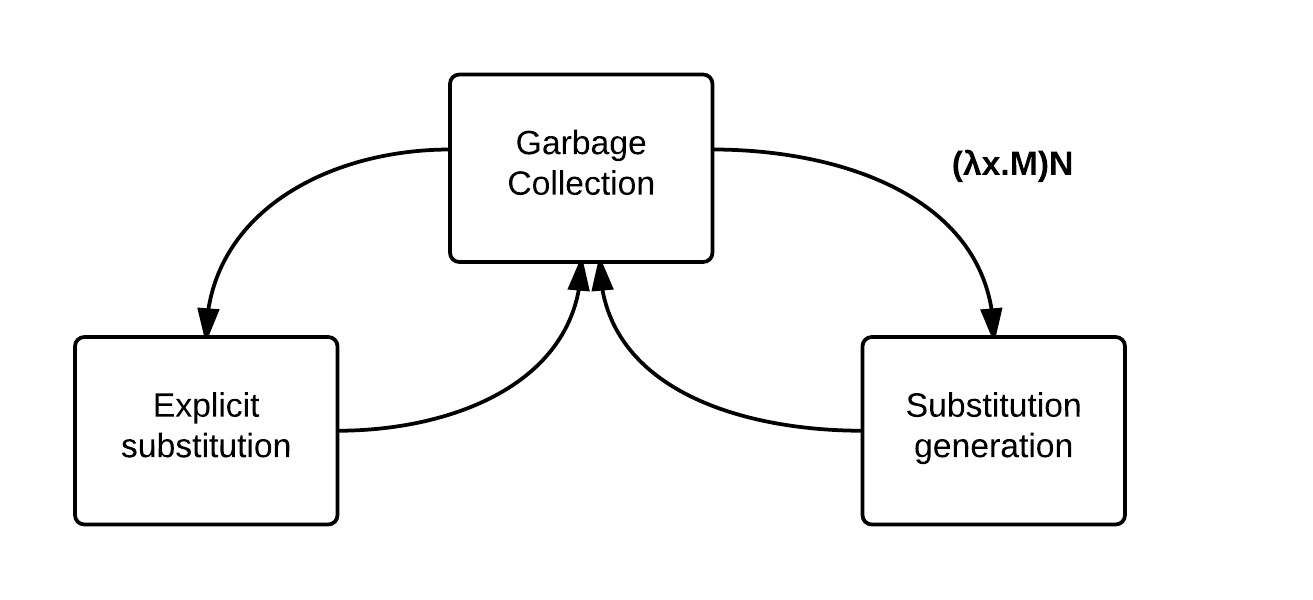
\includegraphics[scale=0.2]{pics/flow}
\caption{Flow chart of $\lambda$xgc-calculus reduction}
\label{fig:flow}
\end{figure}


\begin{figure}[ht]
\centering
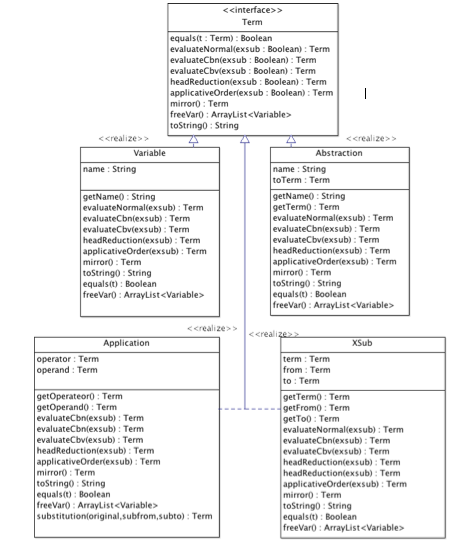
\includegraphics[scale=0.8]{pics/Termxgc}
\caption{Class diagram of $\lambda$xgc-calculus}
\label{fig:termxgc}
\end{figure}
\section{Syntax}

As mentioned before, some parentheses and repeated $\lambda$ are omitted. The input $\lambda$-term should be in the \textbf{most simplified form}. So the $\lambda$-term $((\lambda x.\lambda y.xy)(\lambda f.fx))x$ should be input as \verb|(\xy.xy)(\f.fx)w|. One weakness of the Java implementation in project is that there is no error message displayed on the GUI to tell the user the input is invalid. An application as $(xy)$ would also be parsed as an error input term since the brackets are redundant. Therefore, the user should be careful when input the lambda term. Following are error inputs in general form and their correct format:

\begin{equation*}
     (MN) \rightarrow MN\ \ \ \ \ \ \ \ \ \ (MN)P\rightarrow MNP
\end{equation*}
\begin{equation*}
     (\lambda x.\lambda y.xy) \rightarrow \lambda xy.xy
\end{equation*}



 


